% Created 2023-12-19 Tue 11:22
\documentclass[9pt, b5paper]{article}
\usepackage{xeCJK}
\usepackage[T1]{fontenc}
\usepackage{bera}
\usepackage[scaled]{beraserif}
\usepackage[scaled]{berasans}
\usepackage[scaled]{beramono}
\usepackage[cache=false]{minted}
\usepackage{xltxtra}
\usepackage{graphicx}
\usepackage{xcolor}
\usepackage{multirow}
\usepackage{multicol}
\usepackage{float}
\usepackage{textcomp}
\usepackage{algorithm}
\usepackage{algorithmic}
\usepackage{latexsym}
\usepackage{natbib}
\usepackage{geometry}
\geometry{left=1.2cm,right=1.2cm,top=1.5cm,bottom=1.2cm}
\usepackage[xetex,colorlinks=true,CJKbookmarks=true,linkcolor=blue,urlcolor=blue,menucolor=blue]{hyperref}
\newminted{common-lisp}{fontsize=\footnotesize} 
\author{deepwaterooo}
\date{\today}
\title{ET 框架知识点总结}
\hypersetup{
  pdfkeywords={},
  pdfsubject={},
  pdfcreator={Emacs 29.1 (Org mode 8.2.7c)}}
\begin{document}

\maketitle
\tableofcontents


\section{框架【服务端】启动配置与过程:【亲爱的表哥的活宝妹,任何时候,亲爱的表哥的活宝妹就是一定要、一定会嫁给活宝妹的亲爱的表哥!!!爱表哥,爱生活!!!】}
\label{sec-1}
\begin{itemize}
\item 【亲爱的表哥的活宝妹,任何时候,亲爱的表哥的活宝妹就是一定要、一定会嫁给活宝妹的亲爱的表哥!!!爱表哥,爱生活!!!】
\item Unity 里的应该是【客户端】。
\end{itemize}
\subsection{StartMachineConfig@s.xlsx}
\label{sec-1-1}

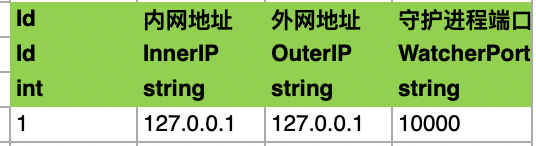
\includegraphics[width=.9\linewidth]{./pic/et6_20231219_111514.png}
\subsection{StartProcessConfig@s.xlsx}
\label{sec-1-2}


\includegraphics[width=.9\linewidth]{./pic/et6_20231219_112239.png}
\subsection{StartSceneConfig@s.xlsx}
\label{sec-1-3}

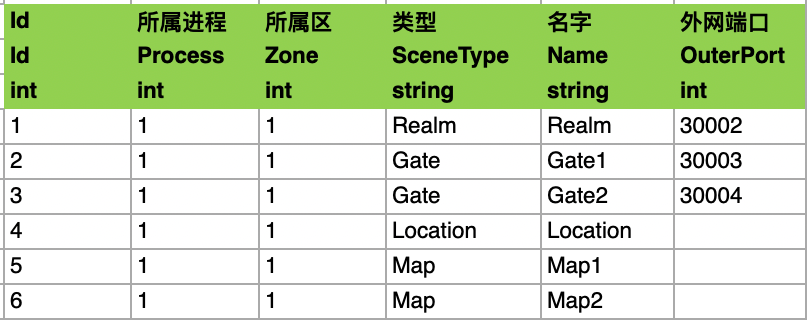
\includegraphics[width=.9\linewidth]{./pic/et6_20231219_111600.png}
\subsection{StartZoneConfig@s.xlsx}
\label{sec-1-4}

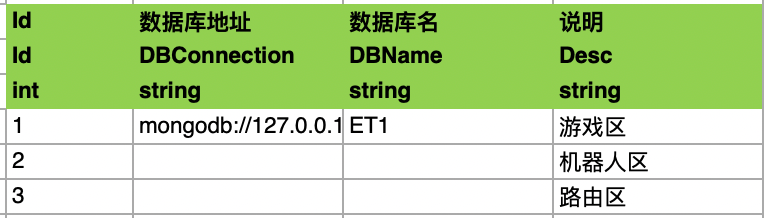
\includegraphics[width=.9\linewidth]{./pic/et6_20231219_111620.png}
\subsection{Simple Summary}
\label{sec-1-5}
\begin{itemize}
\item Unity 里的应该是【客户端】。这几个配置文件放一起,至少,客户端的启动过程是:
\begin{itemize}
\item 一台【物理机 127.0.0.1】;
\item 一个【进程】;
\item 此进程上6 个场景:一个Realm 注册登录服,一个Location 位置管理服,2 个网关服,2 个地图服;
\item 三个区:游戏区,机器人区、路由区。感觉这个区的划分,主要或是仅只与, mongoDb 数据库相关
\end{itemize}
\end{itemize}
% Emacs 29.1 (Org mode 8.2.7c)
\end{document}